\section{Detection and timing}
\label{sec:detect}

\begin{figure*}[t]
\centering
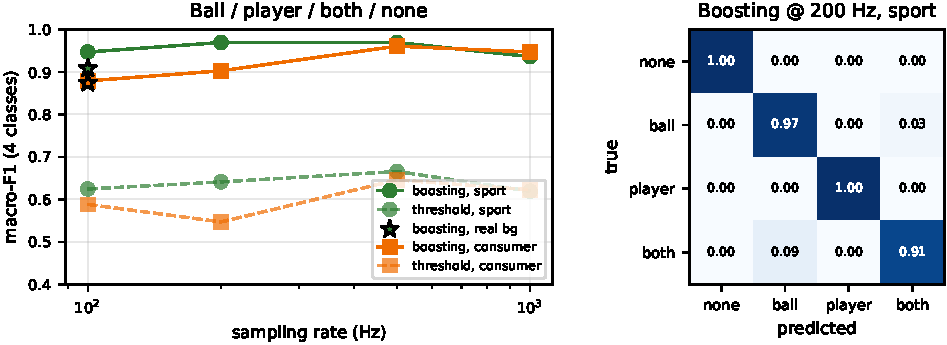
\includegraphics[width=\textwidth]{figures/detect.pdf}
\caption{Left: four-class macro-F1 versus sampling rate for the boosting
classifier (solid) and the tuned threshold rule (dashed), for an impact-rated
(green) and a phone-grade $\pm16$\,g (orange) sensor on synthetic background;
stars are boosting on real PAMAP2 ankle-IMU background at its native 100\,Hz.
Right: the boosting confusion matrix at its best rate. The only systematic
confusion is \emph{both} $\to$ \emph{ball}: when the player pulse is faint the
overlap looks like a clean kick.}
\label{fig:detect}
\end{figure*}

\paragraph{Classification.} Figure~\ref{fig:detect} answers the first
question. With \DetNPerClass\ windows per class (\DetNTrain\ train /
\DetNTest\ test), boosting reaches macro-F1 \DetGbFBest\ at
\DetGbFBestFs\,Hz and stays between \DetGbFOneK\ and \DetGbFBest\ across
100--1000\,Hz; the threshold rule, even with its two thresholds tuned, sits at
\DetThrFMin--\DetThrFMax. The gap is not about detecting \emph{that} something
was hit --- both do that --- but about \emph{what}: a single peak-and-width
rule cannot represent ringing, push tails, direction and secondary peaks at
once. The phone-grade sensor clips \DetConsClipPct\% of the ball impacts, and
at 100\,Hz this costs it (F1 \DetConsFHundred), but by 500\,Hz the shape of
the clipped plateau, the ringing and the direction carry enough information to
recover to \DetConsFBest: full scale matters less than sampling rate. On real
ankle-IMU background at 100\,Hz boosting reaches \DetPamGbSport\ (sport) and
\DetPamGbCons\ (consumer), close to the synthetic values at the same rate,
which says the synthetic gait is not making the task artificially easy; the
threshold rule on real background is \DetPamThrSport.

\begin{figure*}[t]
\centering
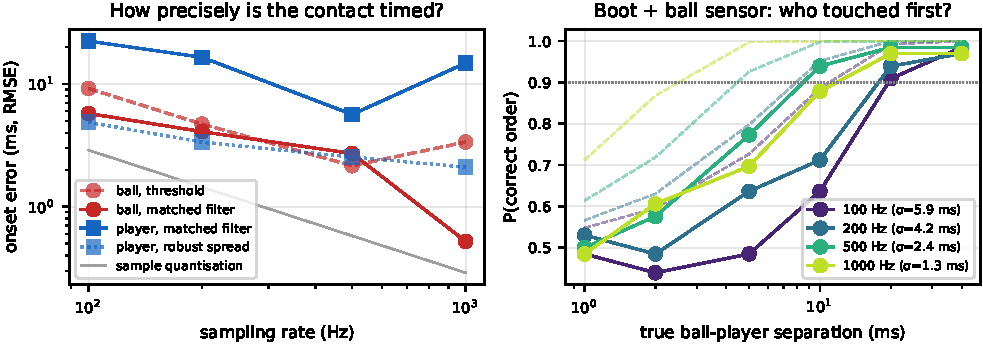
\includegraphics[width=\textwidth]{figures/timing.pdf}
\caption{Left: onset error versus sampling rate (noise at nominal). The ball's
onset follows sample quantisation down to sub-millisecond; the player's RMSE is
dominated by a few gross errors (a faint contact mistaken for a foot strike),
its robust spread is a few ms. Right: probability of correctly ordering a ball
contact and a player contact from the boot's first onset and the ball sensor's
time, versus their true separation, at each rate; dashed lines are the closed
form $\Phi(\Delta/(\sigma\sqrt2))$ with the measured $\sigma$.}
\label{fig:timing}
\end{figure*}

\paragraph{Timing.} The ball onset is timed to \TimBallOneK\,ms RMSE at
1\,kHz, \TimBallFiveH\,ms at 500\,Hz and \TimBallHundred\,ms at 100\,Hz; the
matched filter's parabolic refinement beats the sample grid at high rates,
the threshold crossing is better at low ones (Figure~\ref{fig:timing}, left).
The player onset is intrinsically softer: its robust spread is
\TimPlayerMadOneK\,ms at 1\,kHz but its RMSE (\TimPlayerOneK\,ms) is
dominated by a few percent of gross errors where a weak contact is out-shouted
by a foot strike. Anchoring the estimator on the horizontal component of the
acceleration (foot strikes are vertical) is what brings those gross errors from
tens of percent to a few.

\paragraph{Who touched first, from two clocks.} Given the boot's first onset
and the ball sensor's time, ``ball first'' is declared when the ball fired
within $2\sigma$ of the boot onset, where $\sigma$ combines the boot timing
error with the ball's clock offset and sample quantisation (\OrdSigmaBall\,ms).
The right panel of Figure~\ref{fig:timing} plots the empirical probability of a
correct order against the true separation. At 1\,kHz the combined
$\sigma$ is \OrdSigmaOneK\,ms, the order is right in \OrdPTenOneK\ of cases at
10\,ms and passes 90\% at \OrdGapNinetyOneK\,ms; at 100\,Hz
($\sigma=\OrdSigmaHundred$\,ms) it is \OrdPTenHundred\ at 10\,ms. Below
2--3\,ms every rate is at chance (\OrdPTwoOneK\ at 2\,ms, 1\,kHz). The closed
form with independent Gaussian errors is optimistic at small gaps --- the two
onsets are not independent when the pulses overlap, which is the subject of
the next section --- and matches well once the pulses are distinct.
